\section{Základní pojmy z teorie množin}


\begin{definition}
  \textbf{Množina} je souhrn objektů, chápaný jako celek. Tyto objekty nazýváme prvky množiny.
\end{definition}

\begin{pozn}
Množina může být konečná, nekonečná nebo prázdná. Množinu lze zadat výčtem prvků nebo pomocí charakteristické vlastnosti (např. $\left \{ 2k, k \in \mathbb{N}\right\}$).

\end{pozn}

\begin{definition}
  \textbf{Podmnožina} množiny $A$ je taková množina $B$, že všechny její prvky patří do množiny $A$.
\end{definition}

\begin{pozn}
Každá neprázdná množina má dvě \textbf{nevlastní podmnožiny}: množinu prázdnou a sebe sama. Všechny ostatní její podmnožiny nazýváme vlastní.

\end{pozn}
\begin{definition}
  Množiny $A$ a $B$ se rovnají právě tehdy, když $A$ je podmnožinou $B$ a zároveň $B$ je podmnožinou $A$.
\end{definition}

\begin{definition}
  Nechť $A \subseteq B$ a $B\neq \emptyset$. Množinu všech prvků množiny $B$, které nepatří do množiny $A$, nazýváme \textbf{doplněk} (komplement) množiny $A$ v množině $B$. Značíme $A_B^\prime.$
\end{definition}

\begin{definition}
  Nechť $A, B$ jsou dvě množiny. Jejich \textbf{sjednocením} nazveme takovou množinu, která obsahuje ty prvky, které patří alespoň do jedné z množin $A, B$. Zapisujeme $A \cup B$.
\end{definition}

\begin{definition}
  Nechť $A, B$ jsou dvě množiny. Jejich \textbf{průnikem} nazveme takovou množinu, která obsahuje ty prvky, které patří zároveň do obou těchto množin $A, B$. Zapisujeme $A \cap B$.
\end{definition}

\begin{definition}
  Dvě množiny jsou \textbf{disjunktní}, pokud nemají žádný společný prvek, tedy pokud je jejich průnikem prázdná množina.
\end{definition}

\begin{definition}
  Nechť $A, B$ jsou dvě množiny. \textbf{Rozdíl} množin je množina, která obsahuje všechny prvky množiny $A$ s výjimkou těch, jež jsou zároveň prvky množiny $B$. Zapisujeme $A \smallsetminus B$, někdy též $A-B$.
\end{definition}

\begin{definition}
  \textbf{Vennův diagram} je grafické schematické znázornění všech možných vztahů (sjednocení, průnik, rozdíl, doplněk) několika podmnožin univerzální množiny, jež znázorňujeme pomocí uzavřených čar.
\end{definition}

\begin{veta}[De Morganova pravidla]
  Nechť $A, B$ jsou dvě množiny, $X^\prime$ značí doplněk množiny $X$. Potom platí
  \begin{align*}
  (A \cup B)^\prime &= A^\prime \cap B^\prime, \\
  (A \cap B)^\prime &= A^\prime \cup B^\prime.
  \end{align*}
\end{veta}

\begin{proof}
  Důkaz prvního vztahu:

  \begin{minipage}{0.5\textwidth}
    \centering
        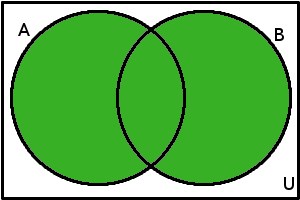
\includegraphics[width=0.5\linewidth]{vennsjed.png}
        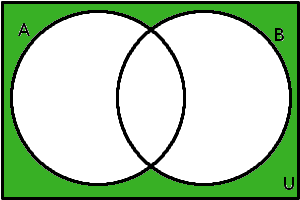
\includegraphics[width=0.5\linewidth]{venndoplsjed.png}
  \end{minipage}
  \hfill
  \noindent\begin{minipage}{0.5\textwidth}
  \centering
        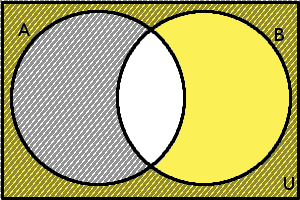
\includegraphics[width=0.5\linewidth]{venndoplAaB.png}
        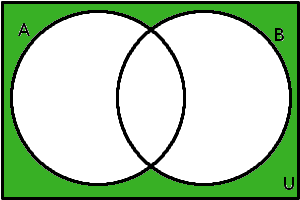
\includegraphics[width=0.5\linewidth]{venndoplsjed.png}
  \end{minipage}

  Důkaz druhého analogicky.
\end{proof}

\begin{pozn}[Číselné množiny]
  Rozlišujeme následující základní číselné množiny:
  \begin{itemize}
    \item $\mathbb{N}$: přirozená čísla $(1, 2, 3, \dots)$,
    \item $\mathbb{Z}$: celá čísla $(\dots, -2, -1, 0, 1, 2, \dots)$,
    \item $\mathbb{Q}$: racionální čísla $(\frac{3}{5}, 0,\overline{3})$,
    \item $\mathbb{R}$: reálná čísla $(e, \pi)$,
    \item $\mathbb{C}$: komplexní čísla $(3+2i)$.
  \end{itemize}
\end{pozn}

Iracionální čísla ($\mathbb{I}$) jsou doplněk racionálních v $\mathbb{R}$.

\begin{definition}
  \textbf{Přirozená čísla} jsou čísla, která vyjadřují počty prvků množin.
\end{definition}

\begin{definition}
  \textbf{Celá čísla} jsou čísla, která vyjadřují počty prvků množin, čísla k nim opačná a číslo 0.
\end{definition}

\begin{definition}
  \textbf{Racionálním číslem} nazveme takové číslo $a = \frac{k}{l},$ kde $ k, l \in \mathbb{Z}$ a $k,l$ jsou nesoudělná.
\end{definition}

\begin{pozn}
  Čísla zapisujeme pomocí dekadického pozičního systému, a to pomocí číslic 0--9 a chápeme je takto:
  $$4503,6=4\cdot 10^3+5\cdot 10^2 + 0 \cdot 10^1 + 3\cdot 10^0 + 6 \cdot 10^{-1}.$$

  Zápis se skládá z celé části, desetinné čárky a desetinného rozvoje. Každé racionální číslo je v desítkové soutavě vyjádřeno buď ukončeným desetinným rozvojem nebo periodickým rozvojem. Iracionální číslo je vyjádřeno neukončeným neperiodickým rozvojem.
\end{pozn}

\begin{definition}
  \textbf{Reálnými čísly} nazýváme všechna čísla, která jsou velikostmi úseček.
\end{definition}

\begin{definition}
  Nechť $a,b \in \mathbb{R},$ kde $a<b$. Pak množiny takových $x\in \mathbb{R},$ že $a\leq x\leq b$ (resp. $a < x < b$, resp. $a < x$, resp. $a \leq x < b$ atd.) nazýváme uzavřeným (resp. otevřeným, resp. neomezeným zleva otevřeným, resp.zprava uzavřeným, zleva otevřeným atd.) \textbf{intervalem}. Zapisujeme $\left<a,b\right>$ (resp. $\left(a,b\right)$, resp. $(a, \infty)$, resp. $\left<a, b\right)$)
\end{definition}

\begin{definition}
  \textbf{Periodický rozvoj čísla} je desetinný rozvoj, u kterého se za desetinnou čárkou donekonečna opakuje (periodicky opakuje) táž číslice nebo skupina číslic. Opakující se číslice nebo skupina opakujících se číslic se nazývá perioda. Zapisují se tak, že se nad opakující se skupinou napíše pruh:
  $$0,333 … = 0,\overline{3}.$$
\end{definition}

\begin{priklad}
    Zapište zlomkem v základním tvaru číslo $0,\overline{14}.$
\end{priklad}

\begin{reseni}
    Platí
    \begin{align*}
        a&=0,\overline{14}\\
        100a &= 14,\overline{14} \\
        99a &= 14\\
        a &= \frac{14}{99}.
    \end{align*}
\end{reseni}


\begin{pozn}
    Pro definici komplexních čísel viz definici \ref{kompl_c_def}.
\end{pozn}

\begin{comment}


\begin{example}[SÚM 169/8]
  Označme $M$ množinu všech dvojciferných přirozených čísel delitelných šesti a $N$ všechn dělitelů čísla 210, kteří jsou různí od čísla 1 a 210. Určete, která z množin má větší počet prvků, a vypište všechny prvky, které mají obě množiny stejné.
  \begin{align*}
    M & = \left\{12, 18, 24, 30, 36, 42, 48, 54, 60, 66, 72, 78, 84, 90, 96\right\}\\
    210 & = 2\cdot 3 \cdot 5  \cdot 7 \textrm{ -- hledáme násobky všech podmnožin těchto čísel} \\
    N  & = \left\{2,3,5,6,7, 10, 14, 15, 21, 30, 35, 42, 70, 105\right\} \\
    |M| & = 15, |N| = 14, M \cap N = \left\{30, 42\right\}
  \end{align*}

  \rm Množina $M$ má více prvků a společná jsou čísla 30 a 42.
\end{example}

\begin{example}[SÚM 171/26]
  $M$ je množina šech reálných čísel $x$, která splňují nerovnosti $-2<x<5$, $N$ je mn. všech reálných čísel $y$, která splňují nerovnost $|y|<4$. Určete množinu $R=M\cup N$ a $S = M\cap N.$ \hfill $R = (-4,5), S=(-2,4).$
\end{example}

\begin{example}[SÚM 172/29f]
  Znázorněte a určete výsledný interval: $(a,a+2)\cap (a-1,a+1),$ kde $a>0.$\hfill$(a,a+1)$
\end{example}

\begin{example}[SÚM (172/33)]
  Je dána kružnice $k$ se středem v bodě  $S$ a poloměrem $r$. Množinu všech bodů uvnitř kružnice označte $A$. Nakreslete rovnostranný trojúhelník $ESD$, jehož jeden vrchol je ve středu dané kružnice a délky stran jsou rovny velikosti jejího průměru. Množinu vnitřních bodů tohoto trojúhelníka ozn. $B$. Díle sestrojte osu úhlu $ESD$ a množinu bodů této přímky označte $C$. Nakreslete samostatné obrázky pro:
  \begin{itemize}
    \item $(A\cap B)\cup C,$
    \item $(A\cup C) \cap (B\cup C),$
    \item $(A\cap B) \cup (B\cap C),$
    \item $(A\cup C) \cap B$.
  \end{itemize}
\end{example}

\begin{example}[SÚM 173/34]
  Pro která $x$ je interval:
  \begin{enumerate}[a.]
    \item $\left<2x,x+3\right>$ částí intervalu $(2,7)$? \hfill $x \in (1,3)$
    \item $(x,5)$ částí intervalu $\left(-1,x+1\right)$? \hfill $x\in (4,5)$
    \item $(x,x+3)$ částí intervalu $\left<5,8\right>$? \hfill $x=5$
    \item $\left<x,2x-1\right>$ částí intervalu $\left<-2,5\right>$? \hfill $x\in\left<-2,5\right>$
    \item $\left<3x,2x+1\right>$ částí intervalu $(3,6)$? \hfill $x\in \left\{\right\}$
  \end{enumerate}
\end{example}

\begin{example}[SÚM 173/35]
  Nechť $M = (a,b), N = (1,8), Q = (1,5)$. Určete $a,b \in \mathbb{R}$ tak, aby platilo $M\cap N = Q$.\hfill $a\in \left(-\infty, 1\right>, b=5$
\end{example}

\begin{example}[SÚM 173/37*]
  Je dán trojúhelník $ABC$. Uvažujme množinu $M$ všech bodů tohoto trojúhelníka, pro které platí $|AX| \geq |BX| \geq |CX|.$ Pomocí velikosti stran a úhlů troj. $ABC$ vyjádřete podmínky pro to, aby:
  \begin{enumerate}[a.]
    \item $X$ byla pětiúhelník, \hfill $\gamma > 90^\circ, \alpha < \beta$
    \item $X$  je jeden bod, \hfill $\alpha = 90^\circ$
    \item $X$ je prázdná.\hfill $\alpha > 90^\circ$
  \end{enumerate}
\end{example}


\begin{example}[SÚM 174/42]
  Jsou dány množiny $M=\left\{1,2; 3; 4\right\},N=\left\{x;y;z\right\}.$ Uveďte alespoň jeden příklad na zobrazení množiny
  \begin{enumerate}[a.]
    \item $M$ do $N$\hfill $1,2\implies x; 3\implies y; 4 \implies y$
    \item $N$ do $M$ \hfill $x\implies 1,2; y\implies 3; z\implies 3$
    \item $M$ na $N.$ \hfill $1,2\implies x; 3 \implies y; 4 \implies z$
  \end{enumerate}
\end{example}

\begin{example}[SÚM 174/46]
  Kolik je všech zobrazení (pod)množiny $\left\{a,b,c,d\right\}$ do (na) množiny $\left\{1,2\right\}$?\hfill \rm 81
\end{example}

\begin{example}[SÚM 106/20]
  Převeďte na obyčejné zlomky:
  \begin{enumerate}[a.]
    \item $0,\overline{27}$\hfill $\frac{27}{99}=\frac{3}{11}$
    \item $0,\overline{6}$ \hfill $\frac{2}{3}$
    \item $2,\overline{345}$ \hfill $2+\frac{345}{999}=\frac{781}{333}$
    \item $0,\overline{1234}$\hfill $\frac{1234}{9999}$
    \item $0,7\overline{2}$\hfill $\frac{7}{10}+\frac{2}{90}=\frac{13}{18}$
    \item $0,1\overline{36}$\hfill $\frac{1}{10}+\frac{36}{990}=\frac{3}{22}$
    \item $0,7\overline{27}$\hfill $\frac{7}{10}+\frac{27}{990}=\frac{8}{11}$
    \item $3,39\overline{85}$\hfill $3+\frac{39}{100}+\frac{85}{9900}=\frac{33646}{9900}$
  \end{enumerate}
\end{example}

\begin{example}[SÚM 107/21]
  Proveďte:
  \begin{enumerate}[a.]
    \item $0,\overline{4}+0,\overline{12}$ \hfill $\frac{4}{9}+\frac{12}{9}=\frac{16}{9}$
    \item $0,\overline{7}+0,\overline{35}$  \hfill $\frac{112}{99}$
    \item $0,\overline{47}+0,\overline{023}$ \hfill $\frac{5470}{10989}$
    \item $0,\overline{47}+0,0\overline{23}$ \hfill $\frac{493}{990}$
    \item $0,5\overline{354}+0,\overline{85}$\hfill $1,394021\dots$
    \item $2,\overline{35}-1,\overline{231}$\hfill$ \frac{4111}{3663}$
    \item $1,\overline{25}-0,\overline{773}$ \hfill $\frac{5261}{10989}$
  \end{enumerate}
\end{example}

\begin{example}[SÚM 107/22*]
  Proveďte:
  \begin{enumerate}[a.]
    \item $1,\overline{2}\cdot 1,\overline{18}$\hfill $\left(1+\frac{2}{9}\right)\left(1+\frac{18}{99}\right)=\frac{11}{9}\cdot \frac{117}{99}=\frac{13}{9}$
    \item $0,\overline{32}\cdot 1,\overline{3}$\hfill $\frac{128}{297}$
  \end{enumerate}
\end{example}

\begin{example}[SÚM 107/23*]
  Řešte rovnici:
  \begin{enumerate}
    \item $0,\overline{25}x + 0,\overline{31}x = 1,\overline{13}$ \hfill $x=2$
    \item $2,\overline{64}x - 3,\overline{48} = 1,\overline{48}x$  \hfill $x = 3$
  \end{enumerate}
\end{example}

\begin{example}[SMP 140/6abc]
  Pomocí Vennových diagramů zjednodušte zápisy množin: \\
  \begin{minipage}{0.5\textwidth}
    \begin{enumerate}[a.]
      \item $(A \cap B \cap C) \cup [B \cap (A^\prime \cup C)^\prime]$
      \item $[(A \cup B)^\prime \cup (B \cup C)] \cap (C \cup A)$
      \item $[(A \cup B^\prime) \cap C] \cup [(B^\prime \cup A^\prime)^\prime \cap C]$
    \end{enumerate}
  \end{minipage}
  \hfill
  \noindent\begin{minipage}{0.5\textwidth}
      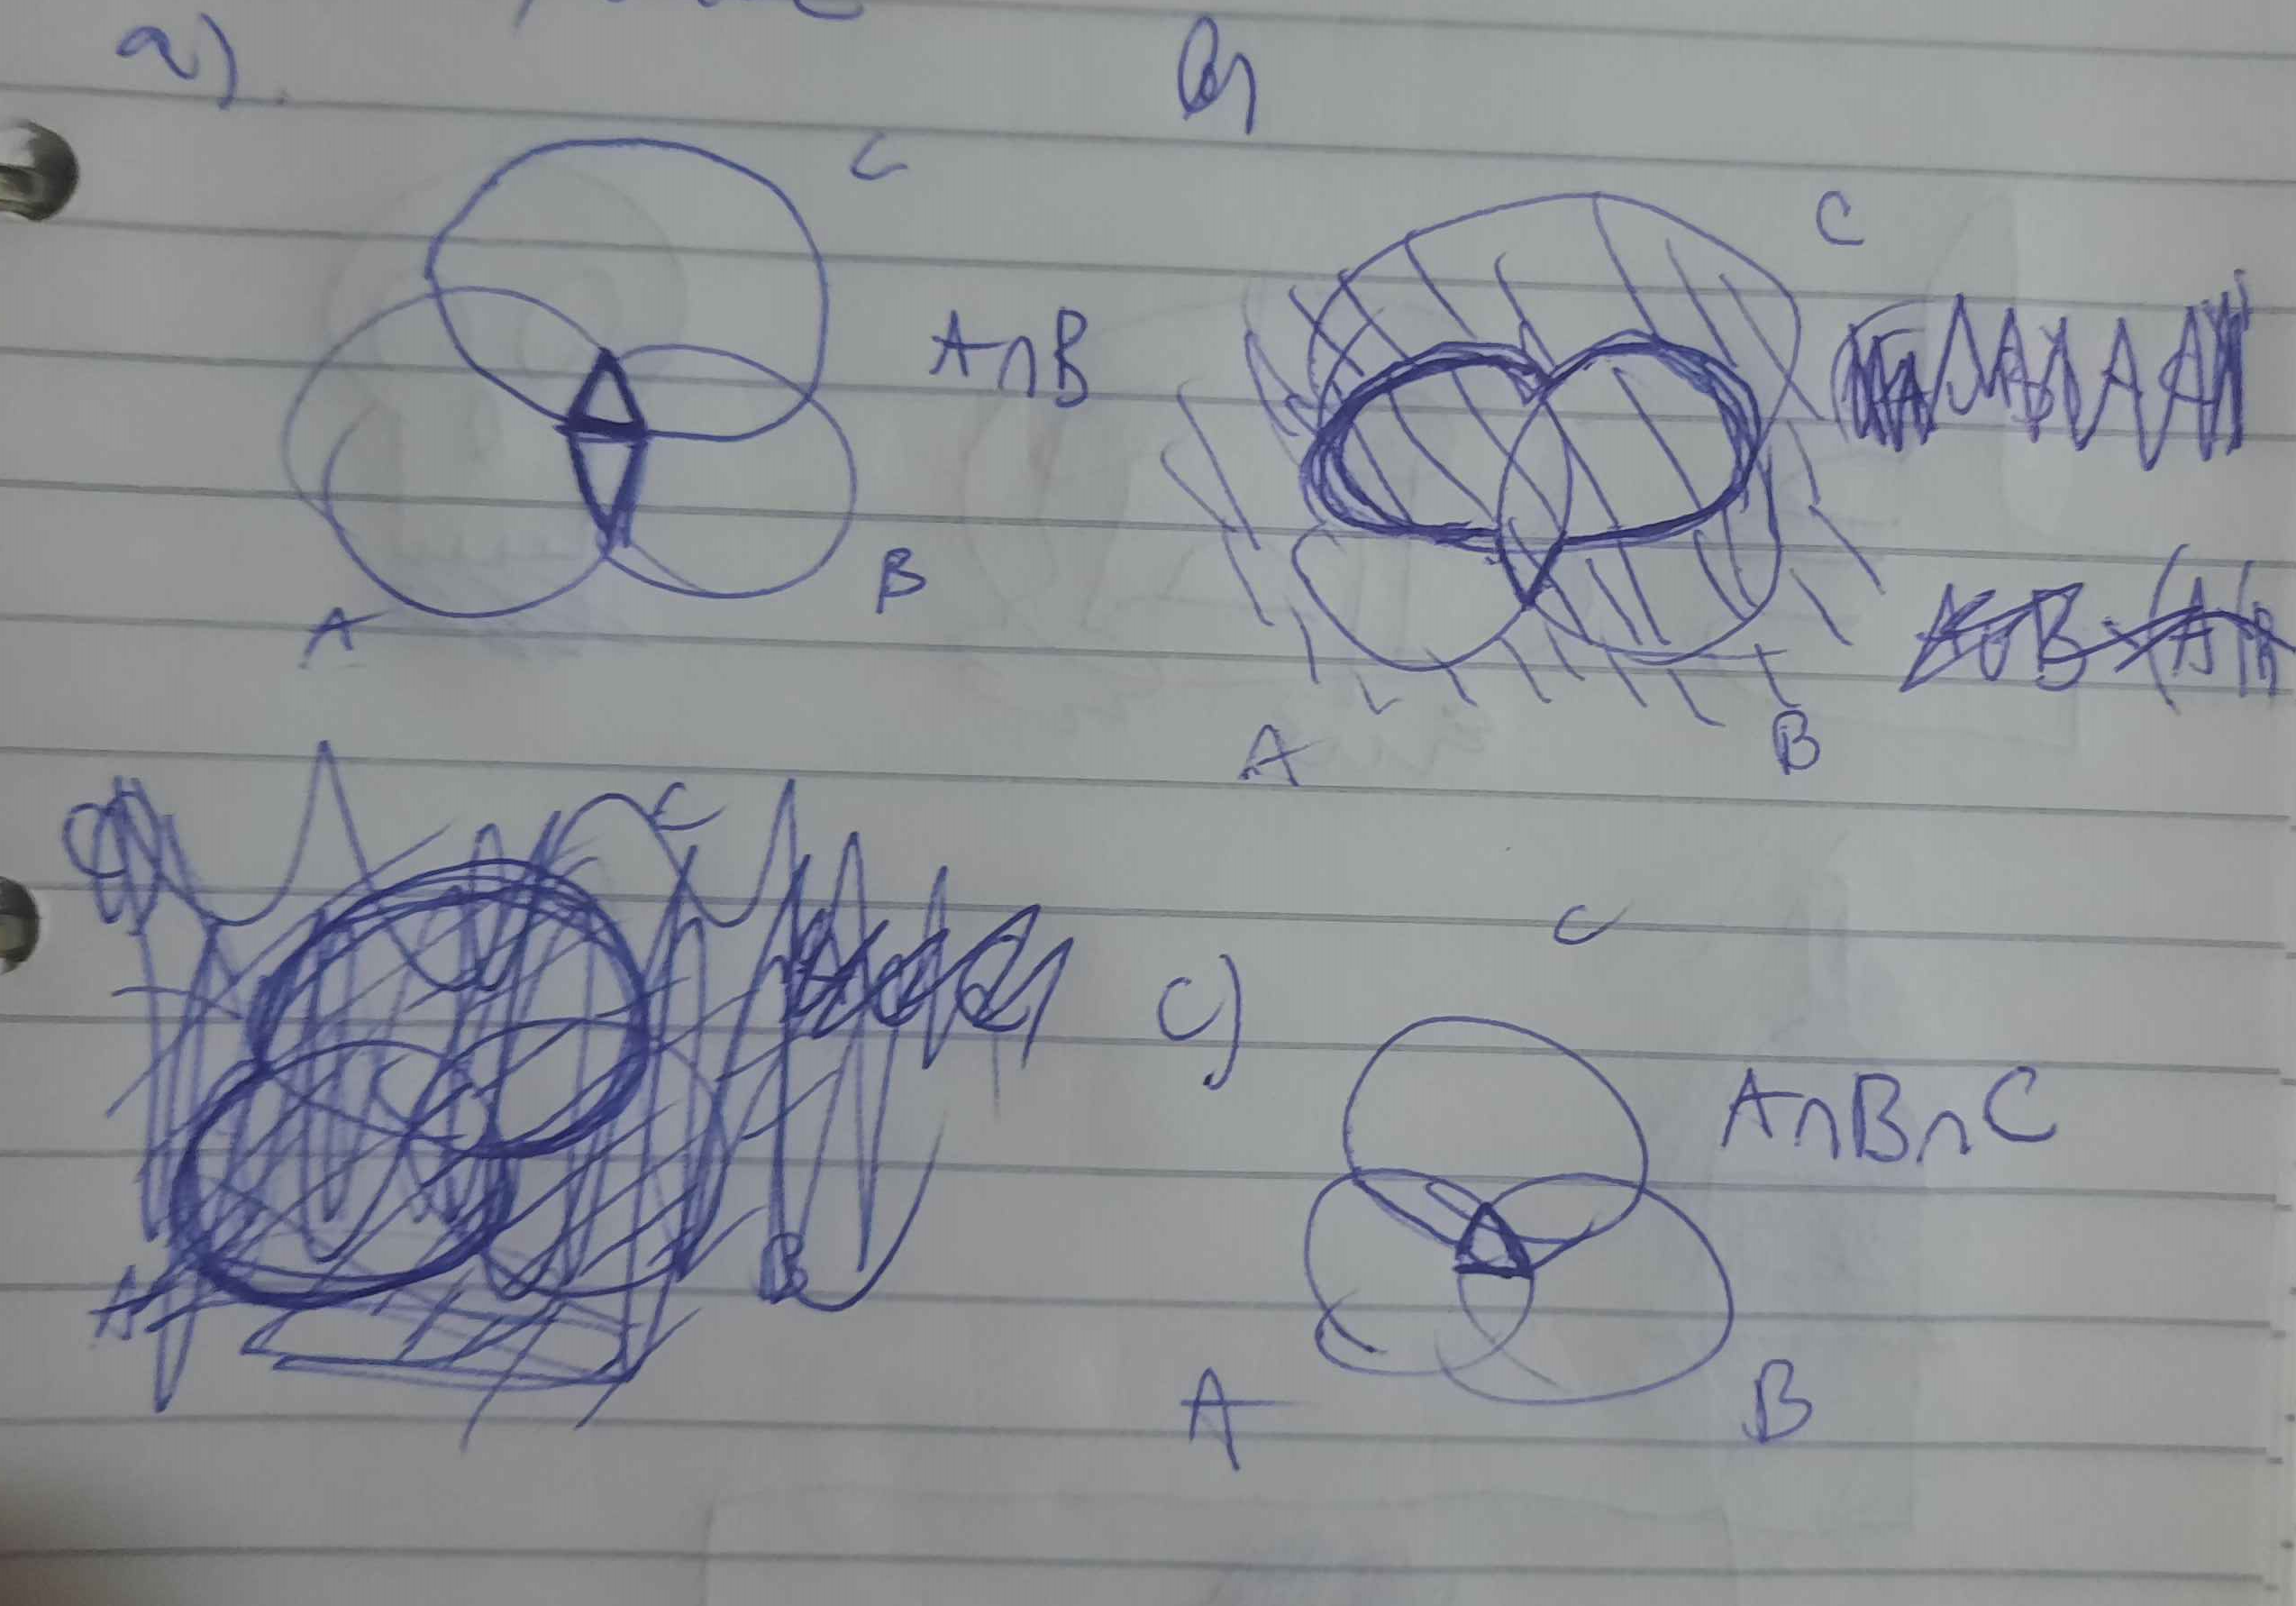
\includegraphics[width=\linewidth]{vennovy}
      \captionof{figure}{}
  \end{minipage}
\end{example}

\begin{example}[SÚM 109/36]
  Dokažte, že číslo $\sqrt{5}$ je iracionální.

  \rm
  Dk. sporem: Nechť $\sqrt{5} \in \Q \implies \sqrt{5} = \frac{a}{b}, a, b \in \Z, D(a, b) = 1$.
  \begin{align*}
    \sqrt{5} & = \frac{a}{b} \\
    5 & = \frac{a^2}{b^2} \\
    5b^2 & = a^2 \implies 5 \mid a^2 \implies 5 \mid a \implies \exists k: a = 5k \\
    5b^2 & = (5k)^2 \\
    5b^2 & = 25k^2 \\
    b^2 & = 5k^2 \implies 5 \mid b^2 \implies 5 \mid b
  \end{align*}
  -- spor s předpokladem, že $D(a, b) = 1 \implies \sqrt{5} \in \mathbb{I}$
\end{example}

\begin{example}[SÚM 109/37]
  Dokažte, že číslo $\sqrt{2} - 1$ je iracionální.

  \rm
  Dk. sporem: Nechť $(\sqrt{2} - 1) \in \Q \implies \sqrt{2} - 1 = \frac{a}{b}, a, b \in \Z, D(a, b) = 1$.
  $$\sqrt{2} - 1 = \frac{a}{b}$$
  $$1 - 2\sqrt{2} = \frac{a^2}{b^2}$$
  $$\frac{b^2-a^2}{2b^2} = \sqrt{2} \implies \sqrt{2} = \frac{p}{q}, p,q \in \Z \implies \sqrt 2 \in \Q \textrm{ -- spor} \implies \sqrt{2} - 1 \in \mathbb{I}$$
\end{example}

\begin{example}[SÚM 109/38]
  Dokažte, že číslo $2\sqrt{5}$ je iracionální.

  \rm
  Dk. sporem: Nechť $2\sqrt{5} \in \Q \implies 2\sqrt{5} = \frac{a}{b}, a, b \in \Z, D(a, b) = 1$.
  $$2\sqrt{5} = \frac{a}{b}$$
  $$10 = \frac{a^2}{b^2}$$
  $$10b^2 = a^2 \implies 10 \mid a^2 \implies 10 \mid a \implies \exists k: a = 10k$$
  $$10b^2 = (10k)^2$$
  $$10b^2 = 100k^2$$
  $$b^2 = 10k^2 \implies 10 \mid b^2 \implies 10 \mid b$$ -- spor s předpokladem, že $D(a, b) = 1$
  $$2\sqrt{5} \in \mathbb{I}$$
\end{example}

\begin{example}[SÚM 109/39]
  Dokažte, že jestliže přirozené číslo $m$ není druhou mocninou žádného přirozeného čísla, potom $\sqrt{m}$ je číslo iracionální.

  \rm
  Dk. sporem: Nechť $m \in \N, m \neq n^2 \forall n \in \N, \sqrt{m} \in \Q \implies \sqrt{m} = \frac{a}{b}, a, b \in \N, D(a, b) = 1$.
  $$\sqrt{m} = \frac{a}{b}$$
  $$m = \frac{a^2}{b^2}, m \in \N \implies b^2 = 1$$
  $$m = a^2, a \in \N$$ -- spor s předpokladem, že $\forall n \in \N: m \neq n^2 $
  QED
\end{example}

\begin{example}[SÚM 144/301]
  Dokažte, že:
  \begin{enumerate}[a.]
    \item součet dvou dvojciferných čísel přirozených, která se liší jen pořadím cifer, je dělitelný jedenácti: $$S = \overline{ab} + \overline{ba} = 10a + b + 10b + a = 11(a + b) \implies 11 \mid S$$
    \item rozdíl dvou dvojciferných čísel přirozených, která se liší jen pořadím cifer, je dělitelný devítí: $$S = \overline{ab} - \overline{ba} = 10a + b - 10b - a = 9(a - b) \implies 9 \mid S$$
    \item rozdíl přirozeného čísla trojciferného  a čísla, které vznikne z tohoto záměnou krajních cifer, je dělitelný 99: $$S = \overline{abc} - \overline{cba} = 100a + 10b + c - 100c - 10b - a = 99(a - c) \implies 99 \mid S$$
  \end{enumerate}
\end{example}

\begin{example}[SÚM 145/303]
  Dokažte, že tři mocniny čísla 2, jejichž exponenty jsou tři po sobě jdoucí přirozená čísla, mají součet dělitelný sedmi: $$S = 2^a + 2^{a+1} + 2^{a+2} = 2^a + 2^a\cdot2^1 + 2^a\cdot2^2 = 7\cdot2^a \implies 7 \mid S$$
\end{example}

\begin{example}[SÚM 145/305]
  Dokažte, že součet třetích mocnin tří po sobě jdoucích přirozených čísel je dělitelný třemi: $$S = a^3 + (a+1)^3 + (a+2)^3 = a^3 + a^3 + 3a^2 + 3a + 1 + a^3 + 6a^2 + 12a + 8 = 3(a^3 + 3a^2 + 5a + 3) \implies 3 \mid S $$
\end{example}

\begin{example}[SÚM 145/306]
  Dokažte, že:
  \begin{enumerate}[a.]
    \item číslo utvořené z rozdílu třetí mociny přirozeného čísla $n$ a tohoto čísla je dělitelné šesti: $$S = n^3 - n = n(n^2-1) = (n-1)n(n+1)$$ \rm Jsou to tři po sobě jdoucí čísla $\implies$ právě 1 z nich je dělitelné třemi $\implies 3 \mid S$
    \item je-li číslo $n$ liché, je uvažovaný rozdíl dělitelný čísel 24: $$S = (n-1)n(n+1)$$ \rm
    Jsou to tři po sobě jdoucí čísla a to prostřední je liché $\implies$ dělitelné třemi, z dalších čísel je jedno dělitelné 2 a jedno dělitelné čtyřmi: $2\cdot4\cdot3 = 24 \implies 24 \mid S$
  \end{enumerate}
\end{example}

\begin{example}[SÚM 145/307]
  Dokažte, že je-li přirozené číslo $x$ liché, je výraz $V = x^3 + 3x^2 — x — 3$ dělitelný číslem 48.

  \rm$$V = x^3 + 3x^2 — x — 3 = x^2(x+3) -(x+3) = (x^2 - 1)(x+3) = (x-1)(x+1)(x+3)$$ $\implies$ tři po sobě jdoucí sudá čísla $\implies$ jedno dělitelné 2, jedno 4 a jedno 6 $\implies 2\cdot4\cdot6 = 48 \implies 48 \mid V$
\end{example}

\begin{example}[SÚM 145/308]
  Dokažte, že výraz $V = 5x^3 + 15x^2 + 10x$ je dělitelný číslem 30 prokaždé přirozené číslo $x$.

  \rm $$V = 5x^3 + 15x^2 + 10x = 5x(x^2 + 3x + 2) = 5x(x+2)(x+1)$$ $\implies$ $x$, $x+1$, $x+2$ tři po sobě jdoucí čísla $\implies$ jedno dělitelné 3, alespoň jedno dělitelné 2, $5x$ dělitelné 5 $\implies 2\cdot3\cdot5=30 \implies 30 \mid V$
\end{example}

\begin{example}[SÚM 145/312]
  Dokažte, že je-li $n$ číslo přirozené, je číslo $N = n^3 + 11n$ dělitelné šesti:

  \rm $\mod 6:$
  \begin{enumerate}
    \item $n = 6k$: $n^3 + 11n \equiv 0^3 + 11\cdot0 \equiv 0 \implies 6 \mid N$
    \item $n = 6k + 1$: $n^3 + 11n \equiv 1^3 + 11\cdot1 \equiv 12 \equiv 0 \implies 6 \mid N$
    \item $n = 6k + 2$: $n^3 + 11n \equiv 2^3 + 11\cdot2 \equiv 30 \equiv 0 \implies 6 \mid N$
    \item $n = 6k + 3$: $n^3 + 11n \equiv 3^3 + 11\cdot3 \equiv 60 \equiv 0 \implies 6 \mid N$
    \item $n = 6k + 4$: $n^3 + 11n \equiv 4^3 + 11\cdot4 \equiv 108 \equiv 0 \implies 6 \mid N$
    \item $n = 6k + 5$: $n^3 + 11n \equiv 5^3 + 11\cdot5 \equiv 180 \equiv 0 \implies 6 \mid N$
  \end{enumerate}
  $\implies 6 \mid N : \forall n \in \N$
\end{example}

\begin{example}[SÚM 145/315]

\end{example}
\end{comment}
